% !TeX root = ../thuthesis-example.tex

\chapter{背景与相关工作}

\section{程序分析与测例构造}

对软件进行测试是提高软件可靠性或寻找潜在漏洞的重要方法,其中关键在于如何编写能覆盖到程序中尽可能多的逻辑,或能触发错误的测例。下面我们在传统程序测试的背景下,结合具体示例,简要介绍三种可用于构造测例的程序分析手段,其中的思想是本文改进计算图生成算法的基础。
待测试程序如代码 \ref{listing:testme} 所示,我们的目标是构造特定的输入组合 $(x, y)$ 以触发第 \ref{listing:testme:bug} 行潜在的除以 0 错误。为了更加清晰地呈现程序的执行过程,我们将第 \ref{listing:testme:bug} 行展开为第 \ref{listing:testme:bugexp:s}-\ref{listing:testme:bugexp:e} 行的逻辑。

\begin{listing}[]
    \caption{存在潜在错误的待测试程序}
    \label{listing:testme}
\begin{minted}[
    fontsize=\small,
    linenos, mathescape, escapeinside=||,
    % texcomments,
    frame=lines,
    framesep=1.5mm,
]{python}
def bbox(v: int) -> int:
    return (v ** 2) % 31

def testme(x: int, y: int) -> int:
    z: int = bbox(x)|\label{listing:testme:bbox}|
    if z == y:|\label{listing:testme:outif}|
        |\label{listing:testme:bug}|# return z // (y - 16)
        if y - 16 != 0: |\label{listing:testme:bugexp:s}|
            return z // (y - 16)
        else:|\label{listing:testme:inelse}|
            raise ZeroDivisionError(
                'divided by `y + 10` which is zero!'
            ) |\label{listing:testme:bugexp:e}|
    return -1
\end{minted}
\end{listing}

\subsection{具体执行}

具体执行意为给程序具体的数值输入,对程序的逻辑与分支进行探索。如输入 $(x, y) = (2, 3)$ ,则 $z = 4, z \neq y$ ,程序无法进入第 \ref{listing:testme:outif} 行的外层分支,更无法进入内层分支以触发错误。可见,随机生成具体测例并具体执行的方式很难实现对程序内的各个分支进行充分探索。

\subsection{符号执行}

符号执行\cite{symbexe}意为不给程序具体的数值输入,而是暂时用符号替代,并维护程序执行到某处时应满足的约束条件。
如令 $(x, y) = (a, b)$ ,则进入第 \ref{listing:testme:outif} 行分支时,程序应满足的条件为 $\texttt{bbox}(a) = b$ 。随后若要进入第 \ref{listing:testme:inelse} 行分支以触发错误,则程序应满足的条件更新为 $\texttt{bbox}(a) = b ~\wedge~ b - 16 = 0$ 。
符号执行利用 SMT(可满足性模理论)求解器对程序应满足的条件进行求解,然而求解器并不支持所有形式的条件。
具体来说,若此处 \texttt{bbox} 返回的是 \texttt{2 * v} ,那么 SMT 求解器可以求解条件 $2a = b ~\wedge~ b - 16 = 0$ ,从而给出可以触发错误的一组输入 $(x, y) = (8, 16)$ 。
而对于代码 \ref{listing:testme} 中的定义, \texttt{bbox} 涉及到了非线性运算(乘方与取模),各种 SMT 求解器要么对这类运算不提供支持,要么很可能运行超时,不能保证给出满足条件的一组解。
更一般地,如果 \texttt{bbox} 的行为没有对应的数学解析式表达,那么更不可能通过用 SMT 求解器求解约束条件来寻找可以触发错误的输入。
总而言之,符号执行对于一些程序可以高效地寻找到能触发错误的输入组合,但受限于 SMT 求解器的能力,不能适用于所有程序。

\subsection{混合执行}

混合执行(concolic execution)\cite{dart, cute}是结合了具体执行(\textbf{conc}rete execution)与符号执行(symb\textbf{olic} execution)执行两种方式的程序分析技术(其英文名词为后两者英文名词的拼接)。对于程序中如 \texttt{bbox} 的复杂部分,混合执行视其为黑盒,用具体执行的方式给定具体输入并获取具体输出,而不用数学表达式描述其行为。
如上例中,输入 $(x, y) = (a, b)$ ,在执行第 \ref{listing:testme:bbox} 行时将 $a$ 具体化为具体数值,如 $4$ ,得到 $z = 16$ 。
接着进入第 \ref{listing:testme:outif} 行的外层分支,此时条件为 $b = 16$ 。然后进入内层第 \ref{listing:testme:bugexp:e} 行的分支,条件更新为 $b = 16 ~\wedge~ b - 16 = 0$ ,调用 SMT 求解器得到 $b = 16$ ,从而找到了能触发错误的输入 $(x, y) = (4, 16)$ 。
当然,若在具体化 $a$ 时赋予了其别的数值,则最终不一定能执行到触发错误的分支。
尽管如此,混合执行只需要具体化 $a$ ,而 $b$ 只需在进入外层分支时参与约束条件,因此分析过程一定能进入外层分支,优于需同时具体化 $a, b$ 而很可能无法进入外层分支的具体执行,也优于可能因为 \texttt{bbox} 的复杂性而止步于第 \ref{listing:testme:bbox} 行的符号执行。
总而言之,混合执行及时随机具体化必要符号以通过代码中的复杂逻辑,相比符号执行拓宽了其所能分析的程序的空间;同时借助了符号化表示与约束求解,相比具体执行有着更强的分支探索能力。

\section{深度学习框架模糊测试}

近年来,对深度学习框架以及编译器的模糊测试工作主要可以被分为两种,分别是用单个算子进行测试,与用多个算子组成的计算图进行测试。接下来,本章将介绍这两种类型下的一些典型工作。

% API-level fuzzing
\subsection{基于单个算子的模糊测试}

单个算子是神经网络的基本组成元素,也是深度学习框架中常用且重要的接口,因此一些现有工作专注于测试主流框架中的单个算子以寻找漏洞,从而提高整体框架的可靠性。

模糊测试工作主要有两大挑战,构造测例与判断正确性。单个算子模糊测试的测例构造需要在输入合法性、算子类型多样性与自动化程度之间权衡取舍。
前人工作 Predoo\cite{predoo} 主要只对 TensorFlow 中的 7 种算子进行测试,如线性层、卷积层、池化层等,通过人工指定几种确定的输入张量与属性参数的组合来构造测例,保证了完全的合法性而牺牲了多样性与自动化程度。对于每个算子, Predoo 比较当输入值受到微小扰动时,其输出值表现的扰动是否在理论推导的上界内,从而寻找潜在漏洞。
FreeFuzz\cite{freefuzz} 为了免于人工构造合法输入带来的低效率问题,通过运行用户文档中的代码片段、开发者编写的单元测试与互联网上的开源项目,并对单个算子的调用接口进行插桩,从而从真实世界代码中收集了大量算子的合法输入组合,并在此基础上进行变异构造,来实现测例的自动获取与生成。对于每个算子, FreeFuzz 比较当输入完全相同时,在不同后端设备(如 CPU 、 GPU)上的输出结果是否一致,通过差分测试寻找潜在漏洞。
DeepREL\cite{deeprel} 在 FreeFuzz 的收集方式之上,使用自然语言处理技术分析用户文档,将所有算子划分为若干等价类,每个等价类中的算子在输入和输出组合上有着某种一致性,因此可以通过比较输出的一致性是否成立来寻找潜在漏洞。对于运行真实世界代码时未收集到任何调用历史的算子, FreeFuzz 无从知晓其合法输入组合,因而无法进行测试;而 DeepREL 可以利用其所在等价类中其它算子的合法输入组合来对其进行测试,从而在不牺牲自动化程度的同时达到了更高的算子类型多样性。

\subsection{基于多算子计算图的模糊测试}

上述针对单个算子的模糊测试工作已经能够较好地覆盖主流深度学习框架中大部分的算子与接口。然而,深度学习框架中的编译器实现了大量计算图层面的优化策略,如常数折叠、算子融合、冗余算子删除等,这些策略无法被只包含单个算子的测例触发。因此,研究者设计并实现了计算图层面的模糊测试,其关键在于在保证计算图合法的前提下,在图的多样性与框架的自动化程度之间进行权衡。

CRADLE\cite{cradle} 直接运行 30 个已有模型进行测试,仅能覆盖 TensorFlow 上的 59 个接口。
在此基础上, LEMON\cite{lemon} 对已有模型进行变异,如在计算图中插入新算子或删除算子,以提高模型多样性。然而,为了维持模型的合法性, LEMON 只能利用不改变张量形状的算子进行变异,而对于卷积层等常常改变张量形状的算子,必须使用固定的参数组合使其不改变张量形状,因此模型多样性受限。
GraphFuzzer\cite{graphfuzzer} 与 Muffin\cite{muffin} 两项工作略微放松了 LEMON 对算子的这一严格限制,而通过添加“填补(padding)”、“切片(slicing)”或“重塑(reshaping)”等额外操作来匹配相邻算子间的张量形状,以进一步提高模型多样性。但这会导致模型中含有大量这类额外操作,与真实世界中人工编写的模型存在较大区别。

NNSmith\cite{nnsmith} 基于符号执行的思想,提出了一种完全符号化的计算图生成算法。首先,它需要人工为 70 余个算子编写符号化规则,包括反映输入张量形状与输出张量形状之间等量关系的形状传播规则,和输入张量形状需要满足的不等式约束条件,从而构建符号化算子集合。其次,它以包含 0 个算子的空计算图为初始,逐个插入符号化算子作为节点,直至图中算子数量达到预定值,得到张量形状均为符号化的计算图。在此过程中,它将根据相邻算子间的张量应满足各自对输入/输出的要求,累积连接关系所形成的符号化约束条件,构建约束条件集合。最后,它调用 SMT (可满足性模理论)求解器寻找满足所有约束条件的一组解,将符号化计算图具体化为张量形状确定的计算图,以作为测试用例。这种先符号化再具体化的生成过程极大地提高了计算图结构与张量形状的多样性,但每个算子均需专家手工编写符号化规则,难以覆盖主流框架中的成百上千种算子与接口,不能高度自动化地达成算子种类的多样性。

% 此外 TZER

% Graph-level fuzzing

% dl systems fuzzing
% compiler fuzzing
% program synthesis
% e-graph, saturation???

\iffalse
而本文正是基于这一观察,提出了一套改进策略,在避免大量人工劳动的前提下将大量 NNSmith 未覆盖到的算子引入到计算图生成中,以对深度学习编译器进行更充分的测试。

\chapter{图表示例}

\section{插图}

图片通常在 \env{figure} 环境中使用 \cs{includegraphics} 插入,如图~\ref{fig:example} 的源代码。
建议矢量图片使用 PDF 格式,比如数据可视化的绘图;
照片应使用 JPG 格式;
其他的栅格图应使用无损的 PNG 格式。
注意,LaTeX 不支持 TIFF 格式;EPS 格式已经过时。

\begin{figure}
  \centering
  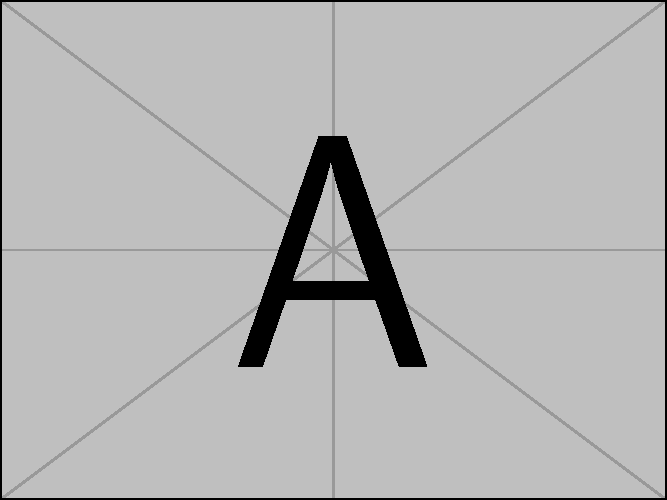
\includegraphics[width=0.5\linewidth]{example-image-a.pdf}
  \caption*{国外的期刊习惯将图表的标题和说明文字写成一段,需要改写为标题只含图表的名称,其他说明文字以注释方式写在图表下方,或者写在正文中。}
  \caption{示例图片标题}
  \label{fig:example}
\end{figure}

若图或表中有附注,采用英文小写字母顺序编号,附注写在图或表的下方。
国外的期刊习惯将图表的标题和说明文字写成一段,需要改写为标题只含图表的名称,其他说明文字以注释方式写在图表下方,或者写在正文中。

如果一个图由两个或两个以上分图组成时,各分图分别以 (a)、(b)、(c)...... 作为图序,并须有分图题。
推荐使用 \pkg{subcaption} 宏包来处理, 比如图~\ref{fig:subfig-a} 和图~\ref{fig:subfig-b}。

\begin{figure}
  \centering
  \subcaptionbox{分图 A\label{fig:subfig-a}}
    {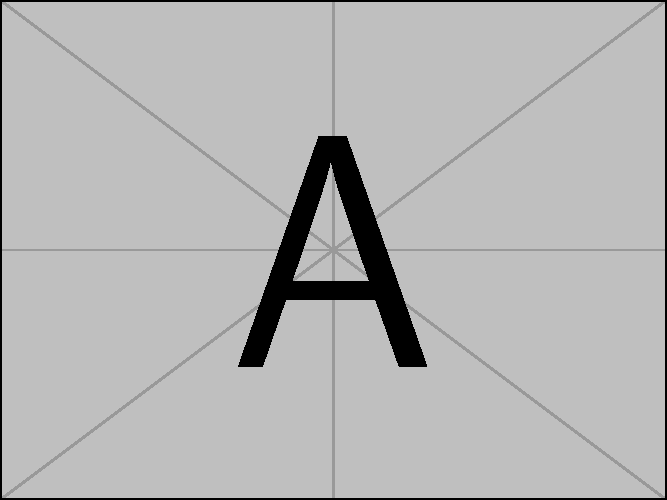
\includegraphics[width=0.35\linewidth]{example-image-a.pdf}}
  \subcaptionbox{分图 B\label{fig:subfig-b}}
    {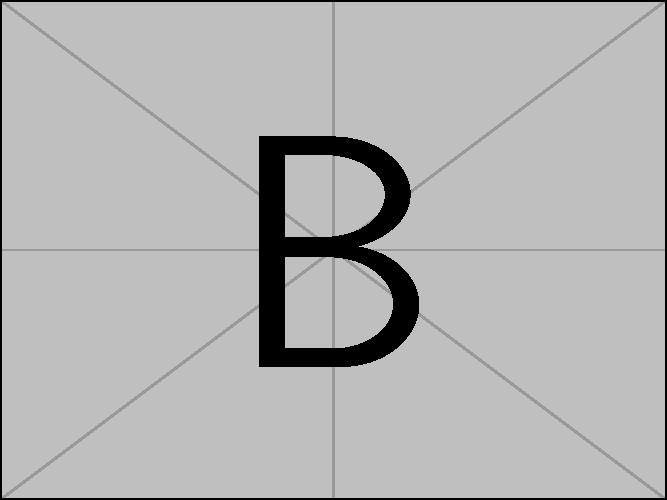
\includegraphics[width=0.35\linewidth]{example-image-b.pdf}}
  \caption{多个分图的示例}
  \label{fig:multi-image}
\end{figure}



\section{表格}

表应具有自明性。为使表格简洁易读,尽可能采用三线表,如表~\ref{tab:three-line}。
三条线可以使用 \pkg{booktabs} 宏包提供的命令生成。

\begin{table}
  \centering
  \caption{三线表示例}
  \begin{tabular}{ll}
    \toprule
    文件名          & 描述                         \\
    \midrule
    thuthesis.dtx   & 模板的源文件,包括文档和注释 \\
    thuthesis.cls   & 模板文件                     \\
    thuthesis-*.bst & BibTeX 参考文献表样式文件    \\
    \bottomrule
  \end{tabular}
  \label{tab:three-line}
\end{table}

表格如果有附注,尤其是需要在表格中进行标注时,可以使用 \pkg{threeparttable} 宏包。
研究生要求使用英文小写字母 a、b、c……顺序编号,本科生使用圈码 ①、②、③……编号。

\begin{table}
  \centering
  \begin{threeparttable}[c]
    \caption{带附注的表格示例}
    \label{tab:three-part-table}
    \begin{tabular}{ll}
      \toprule
      文件名                 & 描述                         \\
      \midrule
      thuthesis.dtx\tnote{a} & 模板的源文件,包括文档和注释 \\
      thuthesis.cls\tnote{b} & 模板文件                     \\
      thuthesis-*.bst        & BibTeX 参考文献表样式文件    \\
      \bottomrule
    \end{tabular}
    \begin{tablenotes}
      \item [a] 可以通过 xelatex 编译生成模板的使用说明文档;
        使用 xetex 编译 \file{thuthesis.ins} 时则会从 \file{.dtx} 中去除掉文档和注释,得到精简的 \file{.cls} 文件。
      \item [b] 更新模板时,一定要记得编译生成 \file{.cls} 文件,否则编译论文时载入的依然是旧版的模板。
    \end{tablenotes}
  \end{threeparttable}
\end{table}

如某个表需要转页接排,可以使用 \pkg{longtable} 宏包,需要在随后的各页上重复表的编号。
编号后跟表题(可省略)和“(续)”,置于表上方。续表均应重复表头。

\begin{longtable}{cccc}
    \caption{跨页长表格的表题}
    \label{tab:longtable} \\
    \toprule
    表头 1 & 表头 2 & 表头 3 & 表头 4 \\
    \midrule
  \endfirsthead
    \caption*{续表~\thetable\quad 跨页长表格的表题} \\
    \toprule
    表头 1 & 表头 2 & 表头 3 & 表头 4 \\
    \midrule
  \endhead
    \bottomrule
  \endfoot
  Row 1  & & & \\
  Row 2  & & & \\
  Row 3  & & & \\
  Row 4  & & & \\
  Row 5  & & & \\
  Row 6  & & & \\
  Row 7  & & & \\
  Row 8  & & & \\
  Row 9  & & & \\
  Row 10 & & & \\
\end{longtable}



\section{算法}

算法环境可以使用 \pkg{algorithms} 或者 \pkg{algorithm2e} 宏包。

\renewcommand{\algorithmicrequire}{\textbf{输入:}\unskip}
\renewcommand{\algorithmicensure}{\textbf{输出:}\unskip}

\begin{algorithm}
  \caption{Calculate $y = x^n$}
  \label{alg1}
  \small
  \begin{algorithmic}
    \REQUIRE $n \geq 0$
    \ENSURE $y = x^n$

    \STATE $y \leftarrow 1$
    \STATE $X \leftarrow x$
    \STATE $N \leftarrow n$

    \WHILE{$N \neq 0$}
      \IF{$N$ is even}
        \STATE $X \leftarrow X \times X$
        \STATE $N \leftarrow N / 2$
      \ELSE[$N$ is odd]
        \STATE $y \leftarrow y \times X$
        \STATE $N \leftarrow N - 1$
      \ENDIF
    \ENDWHILE
  \end{algorithmic}
\end{algorithm}

\fi